\chapter{User Guide}\label{chapter:user-guide}
This manual provides an overview of FuxCP, covering the installation process, its use within OpenMusic and a description of the costs displayed in the interface. Although FuxCP is designed to be compatible with all platforms, it relies on GiL, which currently only works on MacOS and Linux. Unfortunately, GiL does not support Windows due to compatibility issues between the 32-bit Lisp licence used by OpenMusic and the 64-bit Gecode Windows version. Although it is technically possible to obtain a 32-bit version of Gecode for Windows, this is not recommended.

\section{Installing FuxCP}
\subsection{Prerequisites}
To use FuxCP you need to download and install the following tools:
\begin{itemize}
    \item Gecode : \url{https://www.gecode.org/download.html/}
    \item OpenMusic : \url{https://openmusic-project.github.io/openmusic/}
\end{itemize}


And download the following libraries:
\begin{itemize}
    \item GiL : \url{https://github.com/sprockeelsd/GiLv2.0/}
    \item FuxCP : \url{https://github.com/sprockeelsd/Melodizer/}
\end{itemize}
There are other tools available on the latest GitHub, such as Melodizer and Melodizer2.0. For the purposes of this guide, only the FuxCP folder is needed.

\subsection{Loading FuxCP in OpenMusic}
In order to use the above libraries, OpenMusic must be running. When opening any workspace, locate the toolbar at the top of the interface. Click on the "Windows" button, highlighted in the figure~\ref{fig:library}, and select "Library" from the drop-down menu. This will bring up a new window. From the toolbar of this window, select 'File' and then 'Add Remote Library'. Navigate through your file system to find the path where the previously downloaded FuxCP and GiL libraries are stored. Once located, the libraries should appear under the "Libraries" folder in the "Library" window, as shown in Figure~\ref{fig:load}. Right click on "fuxcp" and select "Load Library". If no errors occur, the setup is complete.

However, if an error occurs, it may be a linking problem with the Gecode library. For MacOS users, a script from the \texttt{c++} folder of the GiL library can be used. Edit the path to Gecode within the script to match your system configuration. Linux users should add the Gecode library to the \texttt{LD\_LIBRARY\_PATH} variable. Go to the\newline \texttt{/etc/ld.so.conf.d} folder and create a new \texttt{.conf} file if one does not already exist. In this file, add the full path to the Gecode library, save it, and run \texttt{sudo ldconfig} to update the system with the new library. Don't forget to restart OpenMusic and don't lose hope. Following these steps should ensure that FuxCP works properly.

\begin{figure}[h]
    \centering
    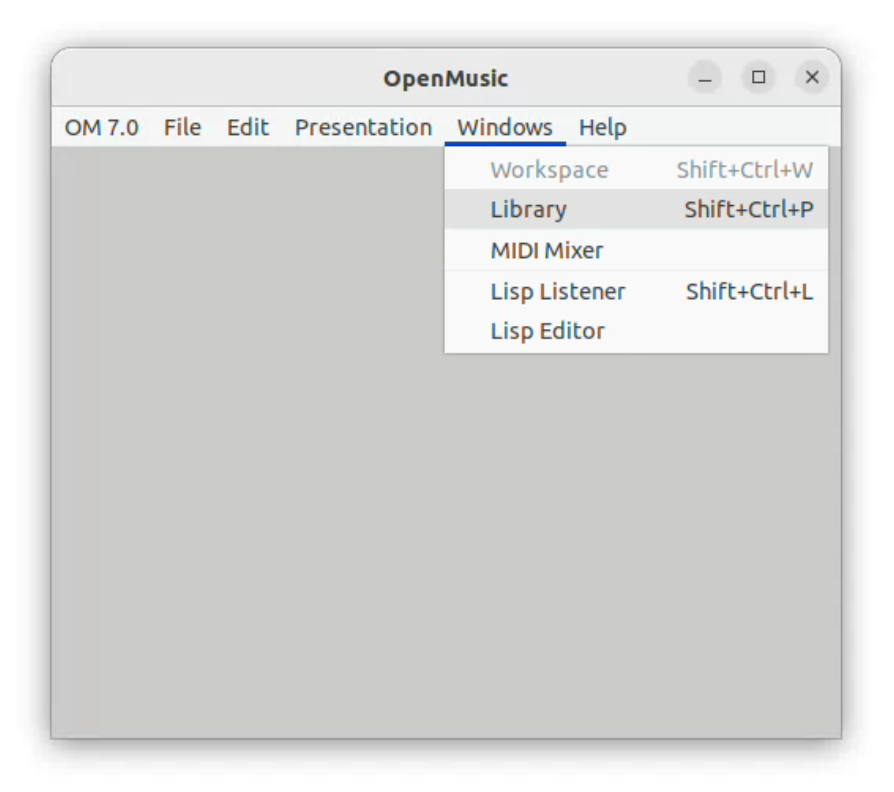
\includegraphics[height=2.6in]{Images/openmusic_library.png}
    \caption{Opening the "Library" window in OpenMusic.}
    \label{fig:library}
\end{figure}
\begin{figure}[h]
    \centering
    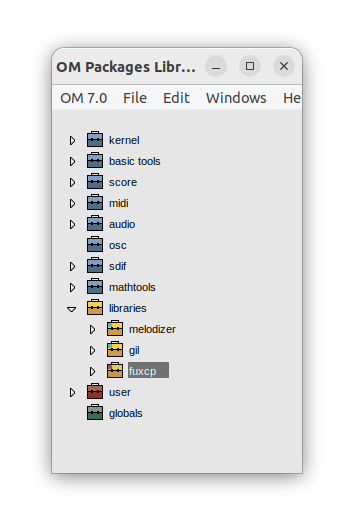
\includegraphics[height=2.6in]{Images/openmusic_load.png}
    \caption{Loading the "fuxcp" library in OpenMusic.}
    \label{fig:load}
\end{figure}

\section{Using FuxCP in OpenMusic}
\subsection*{Setup}
Using FuxCP in OpenMusic is straightforward. There is a single block that contains the entire graphical interface of the tool. This block or class is called \texttt{cp-params}.
\paragraph{Using the example patch}
An example patch, \texttt{FuxCP\_example.omp}, is provided in the 'examples' folder of FuxCP. This patch is the same as the one shown in the figure \ref{fig:om_ext_interface_mod}. To use it, right-click anywhere in the OpenMusic workspace and select $\mathit{Import File}$. Select the sample patch and double-click to open it. Voilà, ready to use!

\paragraph{Setting up your own patch}
If for some reason the example patch is not available, you can set up your own patch as follows. Right-click anywhere in the OpenMusic workspace and select $New...\to New Patch$. Double-click your patch. Once in your patch, right-click anywhere in the patch and select $\mathit{Classes}\to \mathit{Libraries}\to \mathit{FuxCP}\to \mathit{Solver}\to \mathit{CP-PARAMS}$. Alternatively you can just double click anywhere in the patch, type "fuxcp::cp-params" and press enter. This also works for "poly", "voice" and "x-append".

Once this block has appeared, all you have to do is bind an OM voice object, representing the \cfcomma to the second argument of \texttt{cp-params} as shown in figure~\ref{fig:om_ext_interface_mod}. Don't forget to block the input voice object and evaluate \texttt{cp-params} so it can detect the new input. Now \texttt{cp-params} can be blocked too. From now on, you could directly use the interface and generate counterpoints using the tool. If you want to retrieve the voice object containing the counterpoint generated by the tool, just bind the third argument on the output side to a voice object. Once bound, it is then possible to evaluate the voice object so that it updates.

If you want to get the whole composition in one object, you have to do some fiddling with OpenMusic. The simplest way to do this is shown in Figure~\ref{fig:om_ext_interface_mod}, and works as follows: get the POLY object returned by CP-PARAMS on its third output, split this object in two (the two voices), then get the \cfs, which is the second output of CP-PARAMS, and put all the voices back together in the desired order using x-append functions. 

\begin{figure}[h]
  \centering
  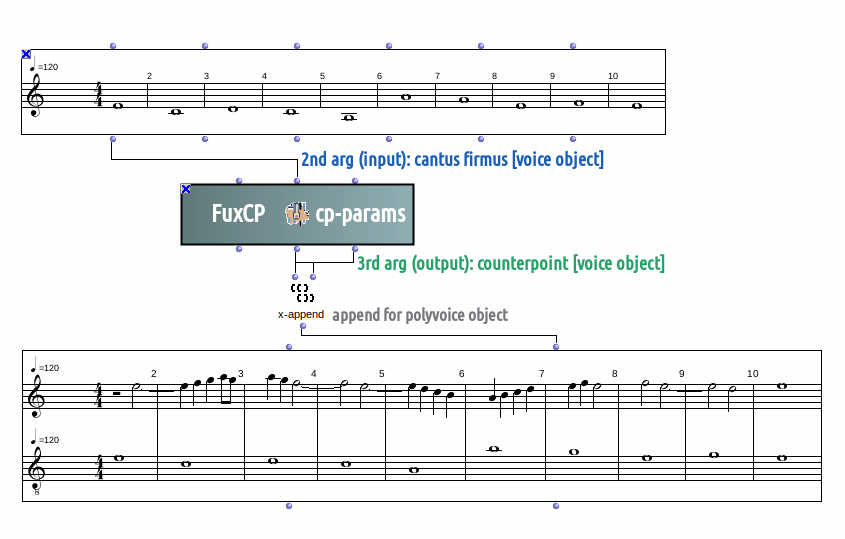
\includegraphics[width=5.2in]{Images/om_ext_interface_mod.png}
  \caption{View of a patch using \texttt{fuxcp::cp-params} in OpenMusic.}
  \label{fig:om_ext_interface_mod}
\end{figure}


\subsection*{Listening to the solution}
OpenMusic does not have built-in sound. You will need to use a third party application to listen to the result. Here is a solution that works to listen to the music: having installed TiMidity++\footnote{TiMidity++ is a software synthesizer that can play MIDI files without a hardware synthesizer, click \href{https://timidity.sourceforge.net/}{here} to install.}, run the following command before opening OpenMusic:


\texttt{timidity -iA -B2,8 -Os}


Then go to $\mathit{OpenMusic} \to \mathit{Preferences} \to  \mathit{MIDI} \to \mathit{Ports\text{ }setup} \to \mathit{Output\text{ }devices}$ and select "TiMidity port 0".


\subsection*{Use the interface}
But how do you use the interface? Simply double-click on the block to bring it up. The interface is sorted from left to right, so the preferences are divided into several categories: "General preferences", "Melodic preferences", "Species-Specific Preferences", "Solver Configuration" and, in the bottom right corner, "Solver Launcher" (see figure~\ref{fig:om_int_interface}). 

\paragraph{Choose the preferences}
You will notice that there are almost always two settings for each preference. The first is the importance: it corresponds to the priority the solver will give to reducing the value of this cost. An importance of $1$ means that it will be the absolute priority of the solver, whereas a preference of $14$ means that the solver will minimise this cost if it doesn't affect the other costs. The second setting is the value: it determines the actual value of the cost corresponding to the preference. It is very useful when two preferences are set to have the same importance, in which case their respective cost values will have an effect. For example, if cost $A$ and cost $B$ both have an importance of $1$, but cost $A$ has a very high cost compared to $B$, $A$ will affect the quality of the solution more than B, even though they both have the same importance. If two costs have the same importance, the yellow panel (bottom left) allows you to choose how to combine them: either by linear combination or by maximum minimisation. For more information, see Chapter~\ref{chapter:search} of this thesis that explains how costs work in detail. The default costs are supposed to represent Fux's preferences.

All costs are explicitly defined in the following section, in Table~\ref{tab:cp-params}.

\paragraph{Start the search}
Pressing the "Next Solution" button will display the solution as a pop-up. What appears on the screen are the two counterpoints. The \cfs must be added manually by using the 'x-append' functions. To see the complete composition, you must evaluate the 'poly' object. To do so, right click on it, and click 'evaluate'. Alternatively, you can click on it and press 'v'.

The other option is to press the "Best Solution" button. This will start an infinite search that will only stop when the best solution has been found (which can take hours). You can evaluate the output object at any time to see what the best result is so far, and this will not stop the search, so you can see how the solution improves step by step, and stop the search when it has produced something you are happy with.

The button "Stop" allows you to stop the search. This button can take up to 5 seconds to actually stop the search. If a search takes too long, we recommend you to stop the search, change the voice range and start again.
Please note that the preferences do not affect the speed of finding the first solution. The first solution is the first valid solution and is not affected by the costs. Only the subsequent solutions can be affected by the preferences.

\begin{sidewaysfigure}
  \centering
  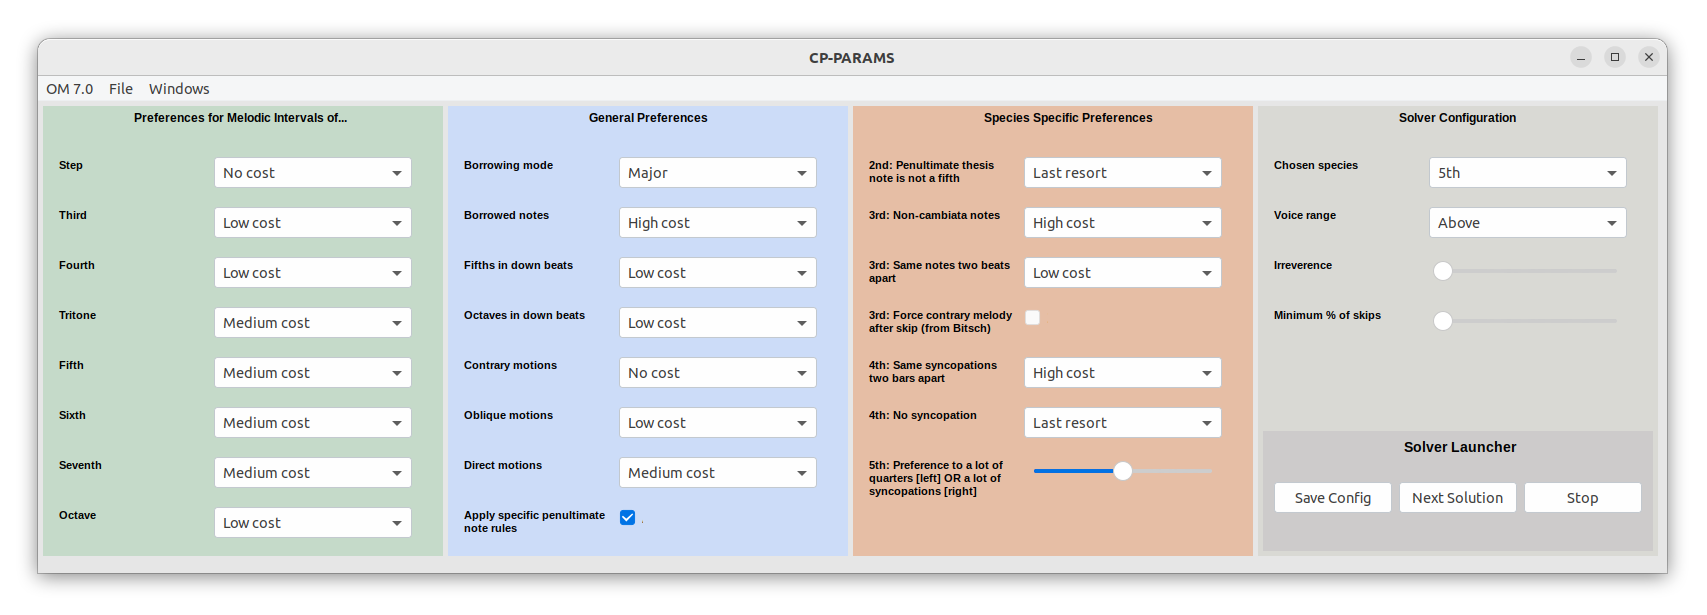
\includegraphics[width=\textheight, height=\textwidth, keepaspectratio]{Images/om_int_interface.png}
  \caption{User interface of the \texttt{fuxcp::cp-params} class in OpenMusic.}
  \label{fig:om_int_interface}
\end{sidewaysfigure}

\section{Interface Parameters Description} \label{appendix:interface-parameters-description}
Table~\ref{tab:cp-params} describes all the parameters available in the interface. A low cost represents a high preference while a high cost represents a low preference.

\begin{table}[h!]
    \footnotesize
    \begin{adjustbox}{center}
        \begin{tabular}{|m{0.22\textwidth}|m{0.82\textwidth}|m{0.15\textwidth}<{\centering}|}
        \hline
        %% GENERAL
        \multicolumn{1}{|c|}{\textbf{Name}} &
          \multicolumn{1}{c|}{\textbf{Description}} &
          \textbf{Default value} \\ \hline
        \cellcolor[HTML]{C8D6FF}Borrowed notes &
          Preference for borrowed notes outside the diatonic scale. A high cost means as few borrowed notes as possible. &
          High cost \\ \hline
        \cellcolor[HTML]{C8D6FF}Harmonic fifths on the downbeat &
          High cost means as few harmonic fifths on the downbeats as possible. &
          Low cost \\ \hline
        \cellcolor[HTML]{C8D6FF}Harmonic octaves on the downbeat &
          High cost means as few harmonic octaves on the downbeats as possible. &
          Low cost \\ \hline
        \cellcolor[HTML]{C8D6FF}Successive perfect consonances &
          High cost means as few successive perfect consonances as possible.&
          Medium cost \\ \hline
        \cellcolor[HTML]{C8D6FF}Repeating notes &
          High cost means as few repeating notes as possible, i.e. as many different notes as possible. This cost corresponds to the variety cost.&
          Medium cost \\ \hline
        \cellcolor[HTML]{C8D6FF}No harmonic triad &
          High cost means as many harmonic triads as possible.&
          Medium cost \\ \hline
        \cellcolor[HTML]{C8D6FF}Direct motion to perfect consonance &
          High cost means as few direct motions to perfect consonances as possible.&
          Last resort \\ \hline
        \cellcolor[HTML]{C8D6FF}Direct motion &
          High cost means as few direct motions as possible. &
          Medium cost \\ \hline
        \cellcolor[HTML]{C8D6FF}Oblique motion &
          High cost means as few oblique motions as possible. &
          Low cost \\ \hline
        \cellcolor[HTML]{C8D6FF}Contrary motion &
          High cost means as few contrary motions as possible. &
          No cost \\ \hline
        \cellcolor[HTML]{C8D6FF}Apply specific penultimate note rules &
          Force all rules on the notes of the penultimate measure. This applies only to two-part composition and  refers to the penultimate note having to be a major sixth or a minor third. &
          Yes \\ \hline
        \hline
        %% MELODIC
        \cellcolor[HTML]{BCE08D}Steps &
          High cost means as few steps as possible. &
          No cost \\ \hline
        \cellcolor[HTML]{BCE08D}Third skips &
          High cost means as few third skips as possible. &
          Low cost \\ \hline
        \cellcolor[HTML]{BCE08D}Fourth leaps &
          High cost means as few fourth leaps as possible. &
          Low cost \\ \hline
        \cellcolor[HTML]{BCE08D}Tritone leaps&
          High cost means as few tritone leaps as possible. &
          Forbidden \\ \hline
        \cellcolor[HTML]{BCE08D}Fifth leaps&
          High cost means as few fifth leaps as possible. &
          Medium cost \\ \hline
        \cellcolor[HTML]{BCE08D}Sixth leaps&
          High cost means as few sixth leaps as possible. &
          Medium cost \\ \hline
        \cellcolor[HTML]{BCE08D}Seventh leaps&
          High cost means as few seventh leaps as possible. &
          Medium cost \\ \hline
        \cellcolor[HTML]{BCE08D}Octave leaps&
          High cost means as few octave leaps as possible. &
          Low cost \\ \hline
        \hline      
        %%% SPECIFIC
        \cellcolor[HTML]{FFCE93}2nd: Penultimate downbeat note is a fifth &
          High cost means trying to ensure that the penultimate downbeat is not a fifth.&
          Last resort \\ \hline
        \cellcolor[HTML]{FFCE93}3rd: No cambiatas &
          A high cost means as many cambiatas as possible &
          High cost \\ \hline
        \cellcolor[HTML]{FFCE93}3rd: Force contrary motion after skip &
          Force that a melodic skip or leap is followed by a melodic step in a contrary motion. &
          No \\ \hline
        \cellcolor[HTML]{FFCE93}3rd: No harmonic triad in 2nd/3rd beat &
          High cost means as many harmonic triads as possible on the 2nd and 3rd beat.&
          Medium cost \\ \hline
        \cellcolor[HTML]{FFCE93}3rd\& 4th: Same note in downbeat and upbeat two beats apart &
          High cost means as many differrent notes in the downbeat and upbeat.&
          Low cost \\ \hline
        \cellcolor[HTML]{FFCE93}4th: No ligatures &
          High cost means as few not-ligatured notes, i.e. as many ligatures as possibles. &
          High cost \\ \hline
        \cellcolor[HTML]{FFCE93}5th: Many quarters or many syncopations &
          Determines the minimum percentage of quarter notes or syncopations in the fifth species. Pushing the slider all the way to one side is not recommended. &
          <center> \\ \hline
        \hline
        %% Solver parameters
        \cellcolor[HTML]{EFEFEF}Voice species &
          Determines the type of counterpoint that the tool will generate. &
          1st and 1st \\ \hline
        \cellcolor[HTML]{EFEFEF}Voice range &
          Determines around which pitch the counterpoint will be generated depending on the pitch of the first note of the \cfdot &
          Above and very far above \\ \hline
        \cellcolor[HTML]{EFEFEF}Minimum \% of skips &
          Determines, depending on the counterpoint size, the percentage of melodic intervals larger than one step. &
          0\% \\ \hline
        \cellcolor[HTML]{EFEFEF}Borrowing mode &
          Type of scale from which notes can be borrowed to generate counterpoint. The first note of the \cfs determines the tonic of this scale. If none is selected, only natural notes are used. Applies everywhere except the penultimate bar. &
          Major \\ \hline
        \cellcolor[HTML]{D1D1D1}Save Config &
          Saves all established preferences and allows you to start a new search for this configuration later. &
          - \\ \hline
        \cellcolor[HTML]{D1D1D1}Next Solution &
          Starts or continues the search for the previously saved configuration. Displays a new window with the first better solution found. Displays an error message if no solution can be found.&
          - \\ \hline
        \cellcolor[HTML]{D1D1D1}Stop &
          Pause the search. This may take up to 5 seconds to take effect. &
          - \\ \hline
        \cellcolor[HTML]{D1D1D1}Best Solution &
          Starts or continues the search for the previously saved configuration. Does not display a window, but returns the best solution found so far, accessible by evaluating the output of \texttt{cp-params}. Displays an error message if no other solution can be found.&
          - \\ \hline
        \hline
        \cellcolor[HTML]{fff078}Linear combination or maximum minimisation &
          Choose whether the equally important costs are combined according to a linear combination or according to a maximum minimisation. More details about it in Chapter~\ref{chapter:search}.&
          Linear combination \\ \hline
        \end{tabular}
    \end{adjustbox}
    \caption{Description of the parameters of \texttt{fuxcp::cp-params}.}
    \label{tab:cp-params}
\end{table}

